% Options for packages loaded elsewhere
\PassOptionsToPackage{unicode}{hyperref}
\PassOptionsToPackage{hyphens}{url}
%
\documentclass[
]{article}
\usepackage{amsmath,amssymb}
\usepackage{lmodern}
\usepackage{ifxetex,ifluatex}
\ifnum 0\ifxetex 1\fi\ifluatex 1\fi=0 % if pdftex
  \usepackage[T1]{fontenc}
  \usepackage[utf8]{inputenc}
  \usepackage{textcomp} % provide euro and other symbols
\else % if luatex or xetex
  \usepackage{unicode-math}
  \defaultfontfeatures{Scale=MatchLowercase}
  \defaultfontfeatures[\rmfamily]{Ligatures=TeX,Scale=1}
\fi
% Use upquote if available, for straight quotes in verbatim environments
\IfFileExists{upquote.sty}{\usepackage{upquote}}{}
\IfFileExists{microtype.sty}{% use microtype if available
  \usepackage[]{microtype}
  \UseMicrotypeSet[protrusion]{basicmath} % disable protrusion for tt fonts
}{}
\makeatletter
\@ifundefined{KOMAClassName}{% if non-KOMA class
  \IfFileExists{parskip.sty}{%
    \usepackage{parskip}
  }{% else
    \setlength{\parindent}{0pt}
    \setlength{\parskip}{6pt plus 2pt minus 1pt}}
}{% if KOMA class
  \KOMAoptions{parskip=half}}
\makeatother
\usepackage{xcolor}
\IfFileExists{xurl.sty}{\usepackage{xurl}}{} % add URL line breaks if available
\IfFileExists{bookmark.sty}{\usepackage{bookmark}}{\usepackage{hyperref}}
\hypersetup{
  pdftitle={Praktická časť diplomovej práce},
  hidelinks,
  pdfcreator={LaTeX via pandoc}}
\urlstyle{same} % disable monospaced font for URLs
\usepackage[margin=1in]{geometry}
\usepackage{color}
\usepackage{fancyvrb}
\newcommand{\VerbBar}{|}
\newcommand{\VERB}{\Verb[commandchars=\\\{\}]}
\DefineVerbatimEnvironment{Highlighting}{Verbatim}{commandchars=\\\{\}}
% Add ',fontsize=\small' for more characters per line
\usepackage{framed}
\definecolor{shadecolor}{RGB}{248,248,248}
\newenvironment{Shaded}{\begin{snugshade}}{\end{snugshade}}
\newcommand{\AlertTok}[1]{\textcolor[rgb]{0.94,0.16,0.16}{#1}}
\newcommand{\AnnotationTok}[1]{\textcolor[rgb]{0.56,0.35,0.01}{\textbf{\textit{#1}}}}
\newcommand{\AttributeTok}[1]{\textcolor[rgb]{0.77,0.63,0.00}{#1}}
\newcommand{\BaseNTok}[1]{\textcolor[rgb]{0.00,0.00,0.81}{#1}}
\newcommand{\BuiltInTok}[1]{#1}
\newcommand{\CharTok}[1]{\textcolor[rgb]{0.31,0.60,0.02}{#1}}
\newcommand{\CommentTok}[1]{\textcolor[rgb]{0.56,0.35,0.01}{\textit{#1}}}
\newcommand{\CommentVarTok}[1]{\textcolor[rgb]{0.56,0.35,0.01}{\textbf{\textit{#1}}}}
\newcommand{\ConstantTok}[1]{\textcolor[rgb]{0.00,0.00,0.00}{#1}}
\newcommand{\ControlFlowTok}[1]{\textcolor[rgb]{0.13,0.29,0.53}{\textbf{#1}}}
\newcommand{\DataTypeTok}[1]{\textcolor[rgb]{0.13,0.29,0.53}{#1}}
\newcommand{\DecValTok}[1]{\textcolor[rgb]{0.00,0.00,0.81}{#1}}
\newcommand{\DocumentationTok}[1]{\textcolor[rgb]{0.56,0.35,0.01}{\textbf{\textit{#1}}}}
\newcommand{\ErrorTok}[1]{\textcolor[rgb]{0.64,0.00,0.00}{\textbf{#1}}}
\newcommand{\ExtensionTok}[1]{#1}
\newcommand{\FloatTok}[1]{\textcolor[rgb]{0.00,0.00,0.81}{#1}}
\newcommand{\FunctionTok}[1]{\textcolor[rgb]{0.00,0.00,0.00}{#1}}
\newcommand{\ImportTok}[1]{#1}
\newcommand{\InformationTok}[1]{\textcolor[rgb]{0.56,0.35,0.01}{\textbf{\textit{#1}}}}
\newcommand{\KeywordTok}[1]{\textcolor[rgb]{0.13,0.29,0.53}{\textbf{#1}}}
\newcommand{\NormalTok}[1]{#1}
\newcommand{\OperatorTok}[1]{\textcolor[rgb]{0.81,0.36,0.00}{\textbf{#1}}}
\newcommand{\OtherTok}[1]{\textcolor[rgb]{0.56,0.35,0.01}{#1}}
\newcommand{\PreprocessorTok}[1]{\textcolor[rgb]{0.56,0.35,0.01}{\textit{#1}}}
\newcommand{\RegionMarkerTok}[1]{#1}
\newcommand{\SpecialCharTok}[1]{\textcolor[rgb]{0.00,0.00,0.00}{#1}}
\newcommand{\SpecialStringTok}[1]{\textcolor[rgb]{0.31,0.60,0.02}{#1}}
\newcommand{\StringTok}[1]{\textcolor[rgb]{0.31,0.60,0.02}{#1}}
\newcommand{\VariableTok}[1]{\textcolor[rgb]{0.00,0.00,0.00}{#1}}
\newcommand{\VerbatimStringTok}[1]{\textcolor[rgb]{0.31,0.60,0.02}{#1}}
\newcommand{\WarningTok}[1]{\textcolor[rgb]{0.56,0.35,0.01}{\textbf{\textit{#1}}}}
\usepackage{longtable,booktabs,array}
\usepackage{calc} % for calculating minipage widths
% Correct order of tables after \paragraph or \subparagraph
\usepackage{etoolbox}
\makeatletter
\patchcmd\longtable{\par}{\if@noskipsec\mbox{}\fi\par}{}{}
\makeatother
% Allow footnotes in longtable head/foot
\IfFileExists{footnotehyper.sty}{\usepackage{footnotehyper}}{\usepackage{footnote}}
\makesavenoteenv{longtable}
\usepackage{graphicx}
\makeatletter
\def\maxwidth{\ifdim\Gin@nat@width>\linewidth\linewidth\else\Gin@nat@width\fi}
\def\maxheight{\ifdim\Gin@nat@height>\textheight\textheight\else\Gin@nat@height\fi}
\makeatother
% Scale images if necessary, so that they will not overflow the page
% margins by default, and it is still possible to overwrite the defaults
% using explicit options in \includegraphics[width, height, ...]{}
\setkeys{Gin}{width=\maxwidth,height=\maxheight,keepaspectratio}
% Set default figure placement to htbp
\makeatletter
\def\fps@figure{htbp}
\makeatother
\setlength{\emergencystretch}{3em} % prevent overfull lines
\providecommand{\tightlist}{%
  \setlength{\itemsep}{0pt}\setlength{\parskip}{0pt}}
\setcounter{secnumdepth}{5}
\ifluatex
  \usepackage{selnolig}  % disable illegal ligatures
\fi

\title{Praktická časť diplomovej práce}
\author{}
\date{\vspace{-2.5em}}

\begin{document}
\maketitle

\hypertarget{sprievodca-ekfmetriou}{%
\section{Sprievodca ekfmetriou}\label{sprievodca-ekfmetriou}}

Sprievodca ekonometriou má za úlohu priblížiť Vám ekonometriu, a pomôcť
Vám jej porozumieť. Sprievodcu píšem ako študent, ktorý sa ekonometriu
začal učiť sám, a sám si prešiel zdĺhavým procesom bádania a
usmerňovania. Sprievodca je zostrojený ako-tak súbežne s osnovou a
zadaniami, ktoré obdržíte na hodine. Nebudeme sa konkrétne držať
vypracovania zadaní, ale skôr princípmi, z ktorých zadania ťažia. Mnoho
študentov tento predmet nezaujíma, a zadania vypracujú okopírovaním
postupov starších spolužiakov, nuž, pochopiť ekonometriu a jej postupy
nie je vôbec jednoduché, a dokážem pochopiť, keď si študenti hľadajú
skratky. Na druhú stranu, ekonometria predstavuje skvelú vstupnú bránu
do sveta analytiky. Človek je zavalený Machine Learningom, Data Sciencom
a AI-čkom, nuž až po sfúknutí pozlátka zistí, že je to zmes matematiky,
štatistiky a počítačovej vedy (CS -- computer science). Ekonometria je
teda skvelou výhovorkou, ako oprášiť matematiku, doučiť sa štatistiku, a
naučiť sa troška programovania. R-ko sa môže zdať ako jazyk, ktorý žije
v tieni Pythonu, avšak, akoby nejedna Dominika vedela povedať, netreba
sa nechať voviesť do omylu. R-ko je najvhodnejší programovací jazyk pre
štatistikov, Google ho zahrnul do najnovších kurzov Google Analytics.
Mojou úlohou je pomôcť Vám prekonať problém, ktorý som na začiatku
svojej cesty ekonometriou vôbec nepovažoval za problém, a to množstvo
materiálov, ktoré zavalí študenta. Pomôžem Vám postupne zložiť skladačku
konceptov a teórií, na ktorých ekonometria stojí. Náročnosť
prezentovania konceptov bude prispôsobená. Nemá zmysel vysvetľovať
odvodzovanie každého estimátora. Cieľom je poskytnúť všeobecný náhľad
ekonometrie, a pomôcť Vám pochopiť, a teda príjemnejšie zvládnuť predmet
Ekonometria.

~

\textbf{Čo nás čaká:}

\begin{itemize}
\tightlist
\item
  Základy programovania v R\\
\item
  Intuitívny prehľad štatistických konceptov\\
\item
  Ekonometrické techniky
\end{itemize}

\newpage

\hypertarget{zuxe1klady-programovania-v-r}{%
\section{Základy programovania v R}\label{zuxe1klady-programovania-v-r}}

\begin{quote}
Sprievodca je interaktívny, teda začneme stiahnutím a inštaláciou
\href{https://cran.r-project.org/mirrors.html}{R} a
\href{https://cran.r-project.org/mirrors.html}{RStudia}. R má samo o
sebe programovacie prostredie, avšak dnešným štandardom je používanie
intregrovaného vývojového prostredia (IDE) v podobe RStudia.
\end{quote}

\hypertarget{aritmetickuxe9-operuxe1tory}{%
\subsection{Aritmetické operátory}\label{aritmetickuxe9-operuxe1tory}}

\emph{Poďme teda rovno na vec. Začneme základnými funkciami.} R môžeme
používať ako kalkulačku, teda za pomoci klasických aritmetických
operátorov môžeme sčítať, odčítať, násobiť, deliť či umocňovať:

\begin{Shaded}
\begin{Highlighting}[]
\DecValTok{5} \SpecialCharTok{+} \DecValTok{5}
\end{Highlighting}
\end{Shaded}

\begin{verbatim}
## [1] 10
\end{verbatim}

\begin{Shaded}
\begin{Highlighting}[]
\DecValTok{5} \SpecialCharTok{{-}} \DecValTok{5}
\end{Highlighting}
\end{Shaded}

\begin{verbatim}
## [1] 0
\end{verbatim}

\begin{Shaded}
\begin{Highlighting}[]
\DecValTok{5} \SpecialCharTok{*} \DecValTok{5}
\end{Highlighting}
\end{Shaded}

\begin{verbatim}
## [1] 25
\end{verbatim}

\begin{Shaded}
\begin{Highlighting}[]
\DecValTok{5} \SpecialCharTok{/} \DecValTok{5}
\end{Highlighting}
\end{Shaded}

\begin{verbatim}
## [1] 1
\end{verbatim}

\begin{Shaded}
\begin{Highlighting}[]
\DecValTok{5}\SpecialCharTok{\^{}}\DecValTok{2}
\end{Highlighting}
\end{Shaded}

\begin{verbatim}
## [1] 25
\end{verbatim}

R-ko dokáže používať aj ďalšie aritmetické operátory:

\begin{Shaded}
\begin{Highlighting}[]
\CommentTok{\# zobrazí zvyšok z delenia}

\DecValTok{5} \SpecialCharTok{\%\%} \DecValTok{2}
\end{Highlighting}
\end{Shaded}

\begin{verbatim}
## [1] 1
\end{verbatim}

My sa budeme zapodievať len tým, s čím sa na cvičeniach stretneme. Našou
úlohou nie je naučiť sa dokonalo ovládať R, ale naučiť sa používať ho v
dostatočnej miere, aby sme s ním zvládli to, čo budeme v najbližšej dobe
potrebovať.

\newpage

\hypertarget{baluxedky}{%
\subsection{Balíky}\label{baluxedky}}

Okrem základných operátorov budeme využívať aj funkcie:

\begin{Shaded}
\begin{Highlighting}[]
\FunctionTok{mean}\NormalTok{(}\DecValTok{2}\NormalTok{, }\DecValTok{4}\NormalTok{, }\DecValTok{6}\NormalTok{)}
\end{Highlighting}
\end{Shaded}

\begin{verbatim}
## [1] 2
\end{verbatim}

\begin{Shaded}
\begin{Highlighting}[]
\FunctionTok{abs}\NormalTok{(}\SpecialCharTok{{-}}\DecValTok{5}\NormalTok{)}
\end{Highlighting}
\end{Shaded}

\begin{verbatim}
## [1] 5
\end{verbatim}

\begin{Shaded}
\begin{Highlighting}[]
\FunctionTok{sqrt}\NormalTok{(}\DecValTok{8}\NormalTok{)}
\end{Highlighting}
\end{Shaded}

\begin{verbatim}
## [1] 2.828427
\end{verbatim}

Tieto funkcie sa nachádzajú v balíkoch, ktoré si môžeme predstaviť ako
také Addony. R figuruje balíkmi, ktoré sú predinštalované, a zahŕňajú
najpoužívanejšie a najzákladnejšie funkcie. Vyššie použíté funkcie sa
nachádzajú v balíku base. To, v akom balíku sa funkcia nachádza zistíte
po napísaní funkcie

~

\begin{center}

\includegraphics{diplomka obrazky/1.png}

\end{center}

~

to však len zapredpokladu, že už máte balík nainštalovaný. Ak narazíte
na názov funkcie, ktorú chcete použiť, avšak nemáte nainštalovaný balík
a chcete zistiť jeho názov, buď si funkciu zadajte do Google, alebo
napíšte do konzoly:

\begin{Shaded}
\begin{Highlighting}[]
\CommentTok{\# ??meno funkcie}

\NormalTok{??mean}
\end{Highlighting}
\end{Shaded}

My budeme často využívať predinštalované balíky \textbf{base} a
\textbf{stats}, avšak za pochodu si budeme inštalovať aj ďalšie balíky,
s ktorými sa na cvičeniach stretnete. Nový balík je potrebné prv
nainštalovať a potom ho načítať do prostredia.

\begin{Shaded}
\begin{Highlighting}[]
\CommentTok{\# stiahneme a našintalujeme pomocou R konzoly a funkcie install.packages()}
\CommentTok{\# ! názov balíka je citlivý na veľkosť písma}
\CommentTok{\# ! názov musí byť v úvodzovkách}

\FunctionTok{install.packages}\NormalTok{(}\StringTok{"fBasics"}\NormalTok{)}

\CommentTok{\# po nainštalovaní máme balík stiahnutý v našom PC, a tento príkaz už viac nepoužívame}
\CommentTok{\# ak však chceme funkcie z balíka použiť, musíme po zapnutí R{-}ka balík načítať príkazom}

\FunctionTok{library}\NormalTok{(fBasics)}

\CommentTok{\# ! tu už úvodzovky nie sú potrebné}
\end{Highlighting}
\end{Shaded}

\begin{quote}
\emph{Pri inštalovaní názov balíka zabalíme do úvodzoviek. Pri jeho
načítaní pomocou library() už úvodzovky nepíšeme. Na pohovor si vezmeme
oblek (úvodzovky), ale po prijatí už chodíme do práce bez obleku.}
\end{quote}

\hypertarget{objekty}{%
\subsection{Objekty}\label{objekty}}

Často chceme vyrátané výsledky znova použiť, a preto by bolo vhodné si
ich niekde uložiť. Na ukladanie a uskladnenie výsledkov slúžia objekty.
Každý objekt má meno a obsah. Meno si môžeme zadať akékoľvek, musí však:

\begin{itemize}
\tightlist
\item
  začínať malým alebo veľkým písmenom a nie číslom
\item
  obsahovať iba čísla, písmená alebo niektoré špeciálne znaky ako
  \("."\) či "\_".
\end{itemize}

\begin{quote}
\emph{Nezabúdajme, že R je case sensitive (rozlišuje veľké a malé
písmená).}
\end{quote}

Povedzme že chceme vytvoriť objekt \textbf{a} a priradiť mu hodnotu
\(2 + 2\). Na priradenie obsahu je možné použiť \("="\), avšak
štandardom je používanie \("<-"\).

\begin{quote}
\emph{Znak \textless- nie je nutné písať dvoma znakmi, používa sa na to
skratka \textbf{``ľavý Alt'' a ``-''}. Na SK klávesnici nájdeme znak
naľavo od pravého Shiftu, na EN klávesnici zvyčajne naľavo od Backspacu.
Osobne programujem s EN klávesnicou, nech som použíteľný v akomkoľvek
štáte bez potreby inštalovať SK klávesnicu.}
\end{quote}

\begin{Shaded}
\begin{Highlighting}[]
\CommentTok{\# Priradíme teda objektu "a" výsledok "2 + 2".}

\NormalTok{a }\OtherTok{\textless{}{-}} \DecValTok{2} \SpecialCharTok{+} \DecValTok{2}

\CommentTok{\# Po napísaní názvu objektu do konzoly nám konzola ukáže už len výsledok.}

\NormalTok{a}
\end{Highlighting}
\end{Shaded}

\begin{verbatim}
## [1] 4
\end{verbatim}

\begin{Shaded}
\begin{Highlighting}[]
\CommentTok{\# Nové priradenie hodnoty starému objektu prepíše starú hodnotu.}

\NormalTok{a }\OtherTok{\textless{}{-}} \DecValTok{5} \SpecialCharTok{+} \DecValTok{5}

\NormalTok{a}
\end{Highlighting}
\end{Shaded}

\begin{verbatim}
## [1] 10
\end{verbatim}

S daným objektom môžeme pracovať, akoby to bola číselná hodnota.

\begin{Shaded}
\begin{Highlighting}[]
\NormalTok{a}\SpecialCharTok{\^{}}\DecValTok{2}
\end{Highlighting}
\end{Shaded}

\begin{verbatim}
## [1] 100
\end{verbatim}

\newpage

\hypertarget{vektory}{%
\subsection{Vektory}\label{vektory}}

Pre priradenie viacerých hodnôt vytvoríme vektor. Vektor vytvoríme
pomocou funkcie c() ako combine.

\begin{Shaded}
\begin{Highlighting}[]
\CommentTok{\# Objektu "a" priradíme súbor číselných hodnôt a vytvoríme z neho vektor.}

\NormalTok{a }\OtherTok{\textless{}{-}} \FunctionTok{c}\NormalTok{(}\DecValTok{5}\NormalTok{, }\DecValTok{1}\NormalTok{, }\DecValTok{4}\NormalTok{, }\DecValTok{2}\NormalTok{, }\DecValTok{3}\NormalTok{)}

\NormalTok{a}
\end{Highlighting}
\end{Shaded}

\begin{verbatim}
## [1] 5 1 4 2 3
\end{verbatim}

S vektormi dokážeme rôzne pracovať. Sčítavať, násobiť, aplikovať na ne
funkcie, všetko, čo nás napadne. Ups, čo nám napadne!

\begin{Shaded}
\begin{Highlighting}[]
\NormalTok{b }\OtherTok{\textless{}{-}} \FunctionTok{c}\NormalTok{(}\DecValTok{5}\NormalTok{, }\DecValTok{9}\NormalTok{, }\DecValTok{6}\NormalTok{, }\DecValTok{8}\NormalTok{, }\DecValTok{7}\NormalTok{)}
\NormalTok{a }\SpecialCharTok{+}\NormalTok{ b}
\end{Highlighting}
\end{Shaded}

\begin{verbatim}
## [1] 10 10 10 10 10
\end{verbatim}

\begin{Shaded}
\begin{Highlighting}[]
\FunctionTok{min}\NormalTok{(a)}
\end{Highlighting}
\end{Shaded}

\begin{verbatim}
## [1] 1
\end{verbatim}

\begin{Shaded}
\begin{Highlighting}[]
\FunctionTok{sort}\NormalTok{(a)}
\end{Highlighting}
\end{Shaded}

\begin{verbatim}
## [1] 1 2 3 4 5
\end{verbatim}

\begin{Shaded}
\begin{Highlighting}[]
\FunctionTok{sum}\NormalTok{(a)}
\end{Highlighting}
\end{Shaded}

\begin{verbatim}
## [1] 15
\end{verbatim}

Je vhodné poznať pár špeciálnych funkcií na tvorbu vektorov. A to:

\begin{Shaded}
\begin{Highlighting}[]
\CommentTok{\# sample(), seq() a rep()}
\end{Highlighting}
\end{Shaded}

Často si totižto potrebujete vytvoriť vektor hodnôt podľa vlastnej
potreby. Hm, to som veľmi nič nové nepovedal. Ale\ldots{} Čo vlastne
tieto funkcie robia? A ako to zistíme? Ak pracujete s úplne novou
funkciou, a máte už nainštalovaný balík, a taktiež ste ho už načítali do
knižnice cez \(library()\), je vhodné použiť \(?názovfunkcie\) alebo
\(help(názovfunkcie)\). Poskytne Vám to stručný popis, čo funkcia robí,
všetky jej argumeny a aj pár príkladov. Ak už ste však s funkciou
pracovali, ale nepamätáte si argumenty, rozpíšte funkciu, kliknite sa do
zátvoriek funkcie \(mean(tu.sa.kliknete)\), a stlačíte \(TAB\). Vyhodí
Vám to argumenty funkcie. Skúsime si to na funkcii \(sample()\).

~

\hypertarget{sample}{%
\subsubsection{sample()}\label{sample}}

\begin{center}
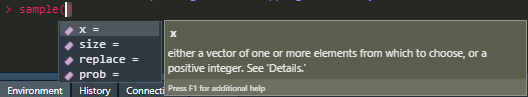
\includegraphics[width=0.85\textwidth,height=\textheight]{diplomka obrazky/2.png}

\end{center}

~

Pri jednej z vecí, ktorú Vám chcem ukázať, budeme potrebovať vektor
výšky ľudí. Tak si ho teda vytvorme už teraz. Ešte predtým môžeme skúsiť
napísať do konzoly \(?sample\), čím zistíme, že funkcia \(sample()\) nám
náhodne vyberie hodnoty zo zadaného vektora.

~

\begin{center}
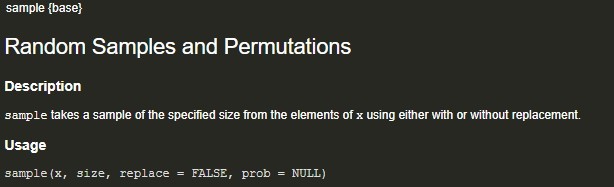
\includegraphics[width=0.8\textwidth,height=\textheight]{diplomka obrazky/3.png}

\end{center}

~

\begin{Shaded}
\begin{Highlighting}[]
\CommentTok{\# Ako prvé potrebujeme zadať "x", teda vektor hodnôt, z ktorých chceme vyberať.}
\CommentTok{\# Pre nás to budú hodnoty medzi 160 až 190, ktoré navolíme ako 160:190.}

\CommentTok{\# 160:190 jednoducho vypíše hodnoty zaradom od 160 do 190. A sample() z nich náhodne vyberie}
\CommentTok{\# nami určený počet hodnôt.}


\CommentTok{\# "size" je počet hodnôt, aký ma funkcia vybrať.}

\CommentTok{\# "replace", či môže vybrať jednu hodnotu viackrát, alebo ju má vylúčiť.}

\CommentTok{\# "prob" použijeme, ak chceme priradiť istým hodnotám inú váhu.}

\NormalTok{vyska }\OtherTok{\textless{}{-}} \FunctionTok{sample}\NormalTok{(}\AttributeTok{x =} \DecValTok{160}\SpecialCharTok{:}\DecValTok{190}\NormalTok{, }\AttributeTok{size =} \DecValTok{10}\NormalTok{, }\AttributeTok{replace =} \ConstantTok{TRUE}\NormalTok{)}

\FunctionTok{print}\NormalTok{(vyska)}
\end{Highlighting}
\end{Shaded}

\begin{verbatim}
##  [1] 187 177 164 160 172 180 168 161 178 168
\end{verbatim}

\begin{quote}
\emph{Funkcia by fungovala, aj keby sme to napísali ako}
``sample(160:190, 10, TRUE)''. \emph{Je však vhodné písať aj argumenty.
Hlavne pri funkciách, ktoré nie sú veľmi bežné. Ak po Vás niekto bude
čítať kód, číta sa to lepšie.}
\end{quote}

\newpage

\hypertarget{seq}{%
\subsubsection{seq()}\label{seq}}

Funkcia \(seq()\) vygeneruje sekvenciu čísel. Ako argumenty zadávame buď
\(od\), \(do\) a \(by\). Teda po akých inkrementoch bude daná sekvencia
narastať.

\begin{Shaded}
\begin{Highlighting}[]
\FunctionTok{seq}\NormalTok{(}\AttributeTok{from =} \DecValTok{2}\NormalTok{, }\AttributeTok{to =} \DecValTok{12}\NormalTok{, }\AttributeTok{by =} \FloatTok{0.5}\NormalTok{)}
\end{Highlighting}
\end{Shaded}

\begin{verbatim}
##  [1]  2.0  2.5  3.0  3.5  4.0  4.5  5.0  5.5  6.0  6.5  7.0  7.5  8.0  8.5  9.0
## [16]  9.5 10.0 10.5 11.0 11.5 12.0
\end{verbatim}

~

\begin{quote}
\emph{V Rku používame na oddeľovanie desatiných miest bodku. Čiarkou
oddeľujeme argumenty. Taktiež nezabúdajte používať medzery. Jedná sa o
gramatiku programovania. Predsalen náš vyššie napísaný výraz vyzerá
lepšie ako} seq(from=2,to=12,by=0.5).
\end{quote}

~

\begin{Shaded}
\begin{Highlighting}[]
\CommentTok{\# Zadáme "od", "do" a koľko časí má vektor mať.}

\FunctionTok{seq}\NormalTok{(}\AttributeTok{from =} \DecValTok{4}\NormalTok{, }\AttributeTok{to =} \DecValTok{10}\NormalTok{, }\AttributeTok{length =} \DecValTok{4}\NormalTok{) }
\end{Highlighting}
\end{Shaded}

\begin{verbatim}
## [1]  4  6  8 10
\end{verbatim}

\begin{Shaded}
\begin{Highlighting}[]
\FunctionTok{seq}\NormalTok{(}\AttributeTok{from =} \DecValTok{4}\NormalTok{, }\AttributeTok{to =} \DecValTok{10}\NormalTok{, }\AttributeTok{length =} \DecValTok{8}\NormalTok{)}
\end{Highlighting}
\end{Shaded}

\begin{verbatim}
## [1]  4.000000  4.857143  5.714286  6.571429  7.428571  8.285714  9.142857
## [8] 10.000000
\end{verbatim}

\begin{Shaded}
\begin{Highlighting}[]
\CommentTok{\# Alternatívou je zadať "od", "po", a rozdeliť to po požadovaných kúskoch}
\CommentTok{\# na požadovanú dĺžku.}

\FunctionTok{seq}\NormalTok{(}\AttributeTok{from =} \DecValTok{4}\NormalTok{, }\AttributeTok{by =} \FloatTok{0.5}\NormalTok{, }\AttributeTok{length =} \DecValTok{25}\NormalTok{)}
\end{Highlighting}
\end{Shaded}

\begin{verbatim}
##  [1]  4.0  4.5  5.0  5.5  6.0  6.5  7.0  7.5  8.0  8.5  9.0  9.5 10.0 10.5 11.0
## [16] 11.5 12.0 12.5 13.0 13.5 14.0 14.5 15.0 15.5 16.0
\end{verbatim}

\hypertarget{rep}{%
\subsubsection{rep()}\label{rep}}

Funkcie \(rep()\) jednoducho zopakuje zadané číslo, alebo vektor,
x-krát.

\begin{Shaded}
\begin{Highlighting}[]
\FunctionTok{rep}\NormalTok{(}\AttributeTok{x =} \DecValTok{1}\NormalTok{, }\AttributeTok{times =} \DecValTok{10}\NormalTok{)}
\end{Highlighting}
\end{Shaded}

\begin{verbatim}
##  [1] 1 1 1 1 1 1 1 1 1 1
\end{verbatim}

\begin{Shaded}
\begin{Highlighting}[]
\FunctionTok{rep}\NormalTok{(}\AttributeTok{x =} \FunctionTok{c}\NormalTok{(}\DecValTok{1}\NormalTok{, }\DecValTok{2}\NormalTok{, }\DecValTok{3}\NormalTok{), }\AttributeTok{times =} \DecValTok{3}\NormalTok{)}
\end{Highlighting}
\end{Shaded}

\begin{verbatim}
## [1] 1 2 3 1 2 3 1 2 3
\end{verbatim}

\hypertarget{indexovanie}{%
\subsection{Indexovanie}\label{indexovanie}}

Indexovanie je v R-ku veľmi užitočný spôsob selektovania dát. Ide
jednoducho o výber súboru dát, zo súboru dát. Indexujeme za použitia
hranatých zátvoriek, ktoré bez medzery nalepíme k objektu, z ktorého
chceme dáta vybrať. Najjednoduchšie sa to vysvetľuje ukážkou. A
nezabúdajte, že R-ko začína od jednotky, nie od nuly. Aj keď nám,
ekonómom neprogramátorom to asi ani nepríde divné.

\begin{Shaded}
\begin{Highlighting}[]
\CommentTok{\# Vytvorme si obyčajný číselný vektor.}

\NormalTok{obycajny\_vektor }\OtherTok{\textless{}{-}} \FunctionTok{c}\NormalTok{(}\DecValTok{1}\SpecialCharTok{:}\DecValTok{10}\NormalTok{)}

\NormalTok{obycajny\_vektor}
\end{Highlighting}
\end{Shaded}

\begin{verbatim}
##  [1]  1  2  3  4  5  6  7  8  9 10
\end{verbatim}

\begin{Shaded}
\begin{Highlighting}[]
\CommentTok{\# Za použitia indexovania môžeme vybrať akúkoľvek hodnotu. Chceme vybrať prvú.}

\NormalTok{obycajny\_vektor[}\DecValTok{1}\NormalTok{]}
\end{Highlighting}
\end{Shaded}

\begin{verbatim}
## [1] 1
\end{verbatim}

\begin{Shaded}
\begin{Highlighting}[]
\CommentTok{\# Alebo súbor hodnôt. Vyberieme prvú a poslednú hodnotu.}

\NormalTok{obycajny\_vektor[}\FunctionTok{c}\NormalTok{(}\DecValTok{1}\NormalTok{, }\DecValTok{10}\NormalTok{)]}
\end{Highlighting}
\end{Shaded}

\begin{verbatim}
## [1]  1 10
\end{verbatim}

Pravdepodobne by väčšina z vás napísala \(obycajny\_vektor[1, 10]\), to
by vám však vyhodilo chybu. Prečo je tomu tak plne pochopíte, keď si
ukážeme matice. Aj keď to nie je nič zložité. Vektor si predstavme ako
šípku, ktorá určuje smer. Je to teda, v našom prípade, reťazec čísel,
jedna dlhá šnúra, ktorá nemá žiadne riadky ani stĺpce. R-ko však to, čo
napíšeme do hranatých zátvoriek vníma ako:

\[[riadok, stĺpec]\]\\
\[[row, column]\]

\begin{quote}
\emph{Zo začiatku sa mi zvyklo pliesť, čo ide prvé. Zapamätal som si to
ako RC autíčko. Také tie malé na ovládanie.}
\end{quote}

Čiže prvý údaj predstavuje riadok, a druhý údaj stĺpec. Ak by sme
napísali \([1, 10]\), R-ko by hľadalo v pŕvom riadku desiatu hodnotu. Do
hranatých zátvoriek píšeme vlastne \textbf{súradnice}. V reťazci hodnôt
máme ale iba reťazec hodnôt. (:D) Preto je potrebné použiť funkciu
\(c()\), aby R-ko vedelo, že má vyberať z reťazca hodnôt. Indexovanie je
veeeľmi užitočné, a dá sa využiť veľmi kreatívne. Nám však stačí vedieť,
čo to plus-mínus robí. Aby ste vedeli, čo sa deje, keď uvidíte hranaté
zátvorky. O indexovaní si ešte povieme pri maticiach.

\begin{Shaded}
\begin{Highlighting}[]
\CommentTok{\# Indexovaním môžeme aj odobrať hodnotu. Napr., ak chceme všetky okrem poslednej:}

\NormalTok{obycajny\_vektor[}\SpecialCharTok{{-}}\DecValTok{10}\NormalTok{]}
\end{Highlighting}
\end{Shaded}

\begin{verbatim}
## [1] 1 2 3 4 5 6 7 8 9
\end{verbatim}

\hypertarget{inuxe9-typy-vektorov}{%
\subsection{Iné typy vektorov}\label{inuxe9-typy-vektorov}}

Vektory nemusia obsahovať len čísla. Môžu obsahovať napríklad aj
\textbf{textové} alebo \textbf{logické} premenné. Existuje ešte aj
štvrtý typ, \textbf{faktorové} vektory, ktorým sa ale nebudeme zaoberať.

\hypertarget{vektor-textovuxfdch-premennuxfdch}{%
\subsubsection{Vektor textových
premenných}\label{vektor-textovuxfdch-premennuxfdch}}

\begin{Shaded}
\begin{Highlighting}[]
\CommentTok{\# Pre vytvorenie vektora obsahujúceho textové reťazce, musí byť obsah ohraničený}
\CommentTok{\# úvodzovkami "".}

\NormalTok{vector\_characters }\OtherTok{\textless{}{-}} \FunctionTok{c}\NormalTok{(}\StringTok{"c"}\NormalTok{, }\StringTok{"musíme"}\NormalTok{, }\StringTok{"používať"}\NormalTok{, }\StringTok{"stále"}\NormalTok{, }\StringTok{"ak"}\NormalTok{, }\StringTok{"chceme"}\NormalTok{,}
                       \StringTok{"viac"}\NormalTok{, }\StringTok{"hodnôt"}\NormalTok{)}

\NormalTok{vector\_characters}
\end{Highlighting}
\end{Shaded}

\begin{verbatim}
## [1] "c"        "musíme"   "používať" "stále"    "ak"       "chceme"   "viac"    
## [8] "hodnôt"
\end{verbatim}

Vektor tvorený textovým reťazcom nájde svoje uplatnenie napríklad pri
pomenovaní hodnôt.

\begin{Shaded}
\begin{Highlighting}[]
\NormalTok{nazvy }\OtherTok{\textless{}{-}} \FunctionTok{c}\NormalTok{(}\StringTok{"prvy"}\NormalTok{, }\StringTok{"druhy"}\NormalTok{, }\StringTok{"treti"}\NormalTok{)}
\NormalTok{cisla }\OtherTok{\textless{}{-}} \FunctionTok{c}\NormalTok{(}\DecValTok{1}\NormalTok{, }\DecValTok{2}\NormalTok{, }\DecValTok{3}\NormalTok{)}

\CommentTok{\# Použijeme na to funkciu names()}

\FunctionTok{names}\NormalTok{(cisla) }\OtherTok{\textless{}{-}}\NormalTok{ nazvy}

\CommentTok{\# Ak sa teraz pozrieme na vektor "cisla", uvidíme, že sme číslam priradili názvy.}
\CommentTok{\# Na vypísanie výsledku môžeme použíť aj funkciu print().}

\FunctionTok{print}\NormalTok{(cisla)}
\end{Highlighting}
\end{Shaded}

\begin{verbatim}
##  prvy druhy treti 
##     1     2     3
\end{verbatim}

Vektor \textbf{``cisla''} sme vlozili do funkcie \textbf{names()}.
Aplikovali sme funkciu na vektor, ktorému sme chceli priradiť názvy.
\textbf{Priradiť}, teda symbol priradenia \textbf{\textless-}, potom už
len vektor s názvami, ktoré chceme priradiť. Pre lepšiu ilustráciu si to
napíšeme nanovo, bez zadefinovaného vektora ``nazvy''.

\begin{Shaded}
\begin{Highlighting}[]
\FunctionTok{names}\NormalTok{(cisla) }\OtherTok{\textless{}{-}} \FunctionTok{c}\NormalTok{(}\StringTok{"adin"}\NormalTok{, }\StringTok{"dos"}\NormalTok{, }\StringTok{"tres"}\NormalTok{)}

\FunctionTok{print}\NormalTok{(cisla)}
\end{Highlighting}
\end{Shaded}

\begin{verbatim}
## adin  dos tres 
##    1    2    3
\end{verbatim}

\newpage

\hypertarget{vektor-logickuxfdch-premennuxfdch}{%
\subsubsection{Vektor logických
premenných}\label{vektor-logickuxfdch-premennuxfdch}}

\begin{Shaded}
\begin{Highlighting}[]
\CommentTok{\# Logické operátory, inak známe ako Booleovské operátory, nám ako výsledok}
\CommentTok{\# poskytnú výstup v podobe TRUE alebo FALSE.}
\CommentTok{\# ! Pre overenie rovnosti použijeme "==".}

\NormalTok{vektor }\OtherTok{\textless{}{-}}  \DecValTok{5}

\NormalTok{vektor }\SpecialCharTok{==} \DecValTok{5}
\end{Highlighting}
\end{Shaded}

\begin{verbatim}
## [1] TRUE
\end{verbatim}

\begin{Shaded}
\begin{Highlighting}[]
\NormalTok{vektor }\SpecialCharTok{==} \DecValTok{6}
\end{Highlighting}
\end{Shaded}

\begin{verbatim}
## [1] FALSE
\end{verbatim}

~

\begin{longtable}[]{@{}ll@{}}
\toprule
Logický operátor & Popis \\
\midrule
\endhead
\textless{} & menšie než \\
\textless= & menšie alebo rovné \\
\textgreater{} & väčšie než \\
\textgreater= & väčšie alebo rovné \\
== & rovná sa \\
!= & nerovná sa \\
!x & nie je x \\
x & y \\
x \& y & x a y \\
isTRUE(x) & test či je x pravdivé \\
\bottomrule
\end{longtable}

~

Logické operátory sa zídu pri indexovaní, alebo pri zisťovaní počtu
vyhovujúcich hodnôt.

\begin{Shaded}
\begin{Highlighting}[]
\CommentTok{\# Vektor výšky ľudí, ktorý sme si skôr vytvorili.}

\NormalTok{vyska }\OtherTok{\textless{}{-}} \FunctionTok{sample}\NormalTok{(}\AttributeTok{x =} \DecValTok{160}\SpecialCharTok{:}\DecValTok{190}\NormalTok{, }\AttributeTok{size =} \DecValTok{10}\NormalTok{, }\AttributeTok{replace =} \ConstantTok{TRUE}\NormalTok{)}

\CommentTok{\# Použitie logického operátora na zistenie, kto má viac ako 170cm. }

\NormalTok{viac\_ako\_170 }\OtherTok{\textless{}{-}}\NormalTok{ vyska }\SpecialCharTok{\textgreater{}} \DecValTok{170}

\CommentTok{\# Výsledky však nebudú číselnými hodnotami, ale hodnotami booleovského typu.}

\FunctionTok{print}\NormalTok{(viac\_ako\_170)}
\end{Highlighting}
\end{Shaded}

\begin{verbatim}
##  [1] FALSE  TRUE  TRUE  TRUE  TRUE FALSE FALSE  TRUE FALSE FALSE
\end{verbatim}

\begin{Shaded}
\begin{Highlighting}[]
\CommentTok{\# To nám však nebráni zužiťkovať to pomocou funkcie "sum()" a zistiť počet }
\CommentTok{\# vyhovujúcich hodnôt. Zráta to všetky TRUE hodnoty.}

\FunctionTok{sum}\NormalTok{(viac\_ako\_170)}
\end{Highlighting}
\end{Shaded}

\begin{verbatim}
## [1] 5
\end{verbatim}

\begin{Shaded}
\begin{Highlighting}[]
\CommentTok{\# Čo dokážeme pomocou indexovania pretvoriť na číselné hodnoty.}

\NormalTok{vyska\_v\_cm }\OtherTok{\textless{}{-}}\NormalTok{ vyska[vyska }\SpecialCharTok{\textgreater{}} \DecValTok{170}\NormalTok{]}

\FunctionTok{print}\NormalTok{(vyska\_v\_cm)}
\end{Highlighting}
\end{Shaded}

\begin{verbatim}
## [1] 186 173 189 178 173
\end{verbatim}

\hypertarget{matice}{%
\subsection{Matice}\label{matice}}

\#nainštalovat len jeden balik a potom ked prejdeme vektory tak c(viac
balikov)

\hypertarget{import-uxfadajov}{%
\subsection{Import údajov}\label{import-uxfadajov}}

Table Header

\begin{longtable}[]{@{}ll@{}}
\toprule
Fukncia & Second Header \\
\midrule
\endhead
Content Cell & Content Cell \\
Content Cell & Content Cell \\
\bottomrule
\end{longtable}

\end{document}
